%%%%%%%%%%%%%%%%%%%%%%%%%%%%%%%%%%%%%%%%
%%%%% NEURAL NETWORK MODELS
%%%%%%%%%%%%%%%%%%%%%%%%%%%%%%%%%%%%%%%%
\section{NEURAL NETWORK MODELS} \label{sec:nn-models}

%%%%%%%%%%%%%%%%%%%%%%%%%%%%%%%%%%%%%%%%
%%%%% SOFTWARE AND HARDWARE USED
%%%%%%%%%%%%%%%%%%%%%%%%%%%%%%%%%%%%%%%%
    \subsection{Software and Hardware Used}
    For defining and training the models, Keras 2.1.4 was used with Tensorflow 1.7 on four AWS Elastic Cloud Compute (EC2) AMI instances. Keras was used in order to streamline the process of creating and defining the neural networks. The loaded music data was split into 90\% training and 10\% validation (the low ratio of validation to training data was due to having a small dataset) and each network was trained on 100 epochs with sample sets being shuffled in between each epoch.
    
    The choice between one or two LSTM layers as well as the input tensor of the network was defined at runtime using parameters passed to the Python script. The following subsections will explain in detail the concept of preparing the input data as well as the exact definitions of 'data vector', 'time steps', 'training samples', and 'input tensor' for the purposes of this paper.
    
%%%%%%%%%%%%%%%%%%%%%%%%%%%%%%%%%%%%%%%%
%%%%% LSTM INPUT STRUCTURE
%%%%%%%%%%%%%%%%%%%%%%%%%%%%%%%%%%%%%%%%
    \subsection{LSTM Input Structure}
     The following algorithm (\ref{alg:load-music}) walks through the pseudocode used to load the audio data into the accepted input tensor based on the parameters passed to the python script.
     
        \begin{algorithm}[h]
            \KwIn{Pre-processed user data, music data location, number of time steps}
            \KwOut{Tensor of dimensions: (training samples, time steps, data vector), Vector or matrix of target values}
            \SetKwProg{function}{load\_music}{end}
            \function{
                $targets$ = empty list\\
                $inputTensor$ = empty list\\
                \ForAll{songs $s$ in $userData$}{
                    $segmentList$ = sorted list of segments in song directory\\
                    $trainingSamplesForSong$ = floor($\frac{\text{length}(segmentList)}{timeSteps}$)\\
                    \For{$i$ in range(0, $trainingSamplesForSong$)}{
                        append $target$ to $targets$\\
                        $currTrainingSample$ = empty list\\
                        $currentClip$ = $i$ * $timeSteps$ \\
                        \For{$j$ in range($currentClip$, $currentClip + timeSteps$)}{
                            load and append column of segment data to $currTrainingSample$
                        }
                     append $currentTrainingSample$ to $inputTensor$ in 3rd dimension  
                    }
                 }
                 \Return $inputTensor$, $targets$
            }
        \caption{Load Music and Target Tensors}
        \label{alg:load-music}
        \end{algorithm}
     
        \subsubsection{Data Vector}
        The phrases 'data vector' or 'clip' refer to the NumPy array of a 5 second audio segment of the song. For example, a 60 second song would be broken up into twelve 5 second clips or data vectors. The reason for this explicit explanation is due to the Keras LSTM input shape definition which uses the phrase 'time steps' to refer to a different concept. In the case that a song was not evenly divisible into 5 second clips, the remainder of the final clip was expanded to 5 seconds by adding silence to the remainder of the clip.
        \subsubsection{Time Steps}
        When calling the Python script to begin training the neural network, the second parameter passed determines the number of time steps that will be used in the network. In this case the phrase 'time step' refers to the number of 5 second clips that are passed as a single training sample to the network. For example, a network with three time steps in the input shape will take in three 5 second clips as a single training sample. In the experiments run, the number of time steps was varied between 1 and 24 as the longest song available was only about 2 minutes long.
        \subsubsection{Training Samples}
        The number of training samples fed into the network was determined by both the number of songs and the length of each individual song. Due to this, each training sample for a single song would be treated as an individual song, except in the case that the song was only long enough to create a single training sample. As an example, if a song was 15 seconds long and the number of time steps was set to 1, then that song would be broken up into 3 training samples, as shown in figure \ref{fig:time-1}. As another example, if a particular song was 45 seconds long and the number of time steps was set to 3, then one would end up with 3 training samples for that song, each with three 5 second clips, as displayed by figure \ref{fig:time-3}, and this song's target would be added 3 times into the targets vector, with each training sample being treated individually.
            \begin{figure}
                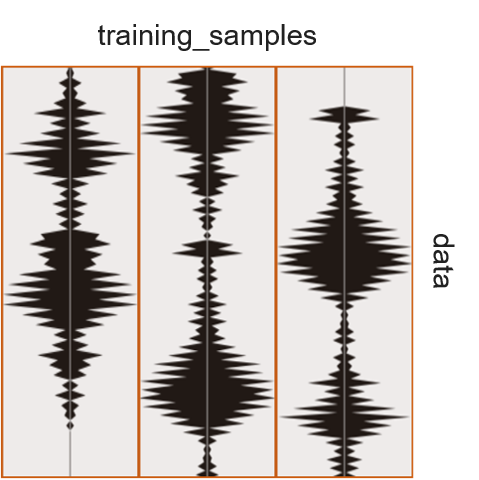
\includegraphics[width=0.45\textwidth]{1_time_step.png}
                \caption{Depiction of Input Using a Single Time Step}
                \label{fig:time-1}
            \end{figure}
            \begin{figure}
                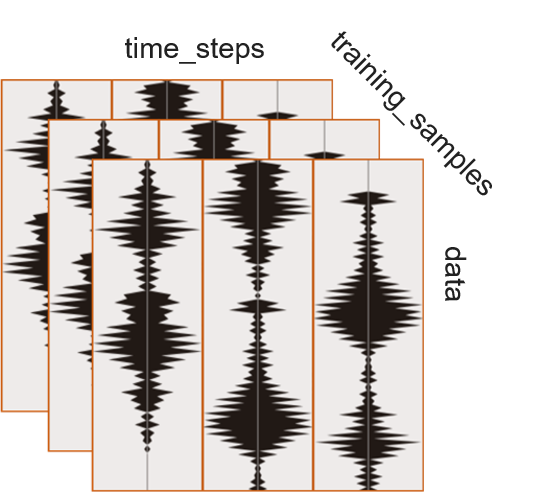
\includegraphics[width=0.45\textwidth]{3_time_steps.png}
                \caption{Depiction of Input Using 3 Time Steps}
                \label{fig:time-3}
            \end{figure}
            
%%%%%%%%%%%%%%%%%%%%%%%%%%%%%%%%%%%%%%%%
%%%%% MODELS USED
%%%%%%%%%%%%%%%%%%%%%%%%%%%%%%%%%%%%%%%%            
    \subsection{Models Used}
    For the experiments, as described at the beginning of the section, two different model shapes were used. First was a single LSTM layer with input shape defined as described previously, followed by a dense layer with a single output node depicted by figure \ref{fig:lstm-1}. The second network architecture used was simply adding another LSTM layer in between the first layer and dense layer as shown in figure \ref{fig:lstm-2}.
            \begin{figure}
                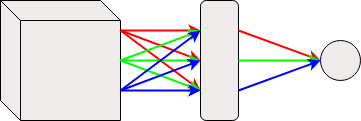
\includegraphics[width=0.45\textwidth]{lstm_single_layer.png}
                \caption{1-Layer LSTM Model}
                \label{fig:lstm-1}
            \end{figure}
            \begin{figure}
                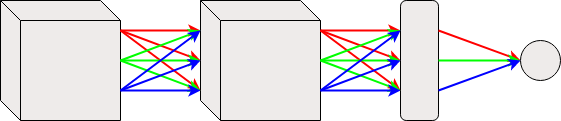
\includegraphics[width=0.45\textwidth]{lstm_2_layer.png}
                \caption{2-Layer LSTM Model}
                \label{fig:lstm-2}
            \end{figure}
